%======================================================================
%----------------------------------------------------------------------
%               XX                              X
%                                               X
%               XX    XXX   XXX   XXX      XXX  X  XXXX
%                X   X   X X   X X   X    X   X X X
%                X   XXXXX XXXXX XXXXX    X     X  XXX
%                X   X     X     X     XX X   X X     X
%               XXX   XXX   XXX   XXX  XX  XXX  X XXXX
%----------------------------------------------------------------------
%  	         A SKELETON FILE FOR IEEE PAPER GENERATION
%----------------------------------------------------------------------
%======================================================================

% first, uncomment the desired options:
\documentclass[%
        %draft,
        %submission,
        %compressed,
        final,
        %
        %technote,
        %internal,
        %submitted,
        %inpress,
        %reprint,
        %
        %titlepage,
        notitlepage,
        %anonymous,
        narroweqnarray,
        inline,
        twoside,
        ]{ieee}
%
% some standard modes are:
%
% \documentclass[draft,narroweqnarray,inline]{ieee}
% \documentclass[submission,anonymous,narroweqnarray,inline]{ieee}
% \documentclass[final,narroweqnarray,inline]{ieee}

% Use the `endfloat' package to move figures and tables to the end
% of the paper. Useful for `submission' mode.
%\usepackage {endfloat}

% Use the `times' package to use Helvetica and Times-Roman fonts
% instead of the standard Computer Modern fonts. Useful for the 
% IEEE Computer Society transactions.
% (Note: If you have the commercial package `mathtime,' it is much
% better, but the `times' package works too).
%\usepackage {times}

% In order to use the figure-defining commands in ieeefig.sty...
\usepackage{ieeefig}

\usepackage{url}

\usepackage{graphicx}

\begin{document}

%----------------------------------------------------------------------
% Title Information, Abstract and Keywords
%----------------------------------------------------------------------
\title[Photon Mapping]{%
       Accurate Radio Transmission Using Photon Mapping}

% format author this way for journal articles.
\author[LaPre \& Anderson]{%
      Justin M. LaPre
      \authorinfo{%
        J. LaPre is a Ph.D. student in the Department of Computer
        Science, Rensselaer Polytechnic Institute, Troy, NY, 12180, USA.}
      \and
      Mark E. Anderson
      \authorinfo{%
        M. Anderson is a Ph.D. student in the Department of Computer
        Science, Rensselaer Polytechnic Institute, Troy, NY, 12180, USA.}
  }

% format author this way for conference proceedings
%\author[SHORT NAMES]{%
%      Mark E. Anderson\member{Fellow}
%      \authorinfo{%
%      Department of Electrical Engineering\\
%      Some University, Somewhere CA, 90210, USA\\
%      Phone: (xxx) xxx-xxxx, email: xxx@xxxx.xxx.xxx}
%    \and
%      Justin M. LaPre\member{Senior Member}
%      \authorinfo{%
%      Department of Electrical Engineering...}
%  }

% specify the journal name
\journal{Advanced Computer Graphics, Spring 2011}

% Or, when the paper is a preprint, try this...
%\journal{IEEE Transactions on Something, 1997, TN\#9999.}

% Or, specify the conference place and date.
%\confplacedate{Troy, NY, USA, May 11, 2010}

% make the title
\maketitle               

% do the abstract
\begin{abstract}
%\section{Abstract}
Accurate simulation of wireless radio signals is a challenging problem.  While
primary effects can easily be calculated, second order effects are numerous
and will often substantially alter the range of the radios.  Many modern
simulators such as ns-3 use a simple, overly conservative calculation known
as the Friis \cite{1697062} equation.

This work demonstrates a more accurate estimate of radio waves via photon
mapping\cite{Jensen96globalillumination}.  By utilizing photon mapping we can
predict where photons
will travel as well as the objects they will strike.  By collecting the number
of photons to strike an object (e.g. an antenna) the effective signal strength
can be determined.  If the signal strength is above a pre-specified cutoff
then the receiving node can hear the transmitter.

We show that this approach generates a higher fidelity estimate in most
scenarios.  As expected, buildings and obstacles impact radio transmissions
in ways that cannot be modeled by the Friis equation.  While the resolution
of radio transmissions is increased, the amount of computation required for
this result has grown considerably, i.e. A straightforward formula has been
replaced with computing the paths of thousands of photons.

%% OLD ABSTRACT

%% Accurate simulation of wireless radio signals is a challenging problem.
%% While primary effects can be easily calculated, second order effects are
%% numerous and will often substantially alter the range of the radios.


%% Simulating wireless networks poses computational problems beyond their wired
%% counterparts.  Determining which nodes are within transmission range of a given
%% node's radio when sending is non-trivial.  Implementing this decision problem
%% in a naive manner will produce an O($n^2$) algorithm.  In a mobile ad-hoc
%% network this would need to be performed before every transmission.

%% Visible light and radio waves are essentially the same phenomenon;
%% we hope to use the abilities of modern GPUs to perform many computations
%% simultaneously to speed up this problem.  McGuire and Luebke
%% \cite{mcguire09imagespace} demonstrated real-time photon mapping
%% of complicated scenes utilizing GPU acceleration.  Schmitz et al.
%% \cite{Schmitz:2006:ERW:1164717.1164730}
%% \cite{Schmitz:2006:WPU:1163610.1163638}
%% improved the accuracy of their ns-2 model via photon mapping.  
%% Simulators such as ROSS \cite{ross} utilize the Transmission Line Matrix
%% \cite{Nutaro:2006:DEM:1138464.1138468} to determine which nodes are able
%% to receive transmissions.  We hope to improve upon both the accuracy and 
%% run-time of TLM in this work.

\end{abstract}
\vspace{5mm}
% do the keywords
\begin{keywords}
wireless networking, 802.11, simulation, photon mapping, ray tracing
\end{keywords}

% start the main text ...
%----------------------------------------------------------------------
% SECTION I: Introduction
%----------------------------------------------------------------------
\section{Introduction}

Wireless radio communication has become ubiquitous and, in fact, necessary for 
many purposes ranging from widespread wifi hot-spots for web browsing to 
critical military applications.  Whether or not one node is capable of 
hearing another is an essential question, the answer to which will 
determine the effective ability to communicate.

Efficiency is critical when establishing a communication mesh between the
nodes. Implementing this decision problem
in a naive manner will produce an O($n^2$) algorithm.  In a mobile ad-hoc
network this would need to be performed before every transmission.

An oracle for deciding whether or not node $x$ can hear node $y$ would be useful 
in this situation.  Unfortunately, such an oracle does not exist and we must 
fall back on approximating an answer.  One such method adopted by ns-2 and 
ns-3 is the Friis \cite{1697062} equation.  The Friis equation assumes
idealized 
conditions and that no other objects interfere with communications.  Clearly 
this is an over-simplification; many materials impact radio wave transmission 
in some, oftentimes significant, manner.

In this work we propose an improved method of approximating radio 
transmissions.  By modeling the radio communications as photons, determining 
the signal strength is simply a matter of gathering photons which impact a 
region of interest.  A variation of photon mapping is applicable in this
scenario.  By enclosing radio receivers in bounding spheres, the number of
photons to impact the sphere and, in turn, the signal strength of the radio
signals, can be determined.

Photon mapping algorithm was developed by Jensen \cite{Jensen96globalillumination} 
to improve upon deficiencies in classic ray tracing approaches.  It is a
realistic two-pass global illumination algorithm which consists of shooting
photons into the scene and then performing a local collection step.

%% \section{Related Work}

%% \begin{enumerate}
%% \item photon mapping

%% \item radio transmission

%% \item radio transmission using photon mapping (like from other papers, e.g. the
%% guys who do the beam stuff)
%% \end{enumerate}

\section{Overview}
Our approach begins by emitting photons from our radio transmitter in a
directional manner.  The output of this transmitter is 250 mW.  We chose this
value in our aim to mimic something along the lines of a typical Wifi base
station such as a Linksys wireless router.

%% /**
%%  * \brief A Friis propagation loss model
%%  *
%%  * The Friis propagation loss model was first described in
%%  * "A Note on a Simple Transmission Formula", by 
%%  * "Harald T. Friis".
%%  * 
%%  * The original equation was described as:
%%  *  \f$ \frac{P_r}{P_t} = \frac{A_r A_t}{d^2\lambda^2} \f$
%%  *  with the following equation for the case of an
%%  *  isotropic antenna with no heat loss:
%%  *  \f$ A_{isotr.} = \frac{\lambda^2}{4\pi} \f$
%%  *
%%  * The final equation becomes:
%%  * \f$ \frac{P_r}{P_t} = \frac{\lambda^2}{(4 \pi d)^2} \f$
%%  *
%%  * Modern extensions to this original equation are:
%%  * \f$ P_r = \frac{P_t G_t G_r \lambda^2}{(4 \pi d)^2 L}\f$
%%  *
%%  * Here, we ignore tx and rx gain and the input and output values are in dB or dBm:
%%  * \f$ RX_{dB} = TX_{dB} + 10\mathrm{log_{10}} \frac{\lambda^2}{(4 \pi d)^2 L}\f$
%%  *
%%  * With:
%%  *  - \f$ P_r \f$ : reception power (W)
%%  *  - \f$ P_t \f$ : transmission power (W)
%%  *  - \f$ G_t \f$ : transmission gain (unit-less) 
%%  *  - \f$ G_r \f$ : reception gain (unit-less)
%%  *  - \f$ \lambda \f$ : wavelength (m)
%%  *  - \f$ d \f$ : distance (m)
%%  *  - \f$ L \f$ : system loss (unit-less)
%%  *
%%  *
%%  * This model is invalid for small distance values.
%%  * The current implementation returns the txpower as the rxpower
%%  * for any distance smaller than MinDistance.
It would be constructive to examine the Friis equation for any possible
simplifying assumtions.  A modern extension to the original Friis equation
\cite{1697062} is
\begin{eqnarray}
P_r = \frac{P_t G_t G_r \lambda^2}{(4 \pi d)^2 L}
\end{eqnarray}
We can assume a unity value for both the transmission gain $G_t$ and reception
gain $G_r$ as ns-3 also makes these assumptions.  This reduces the equation to

\begin{eqnarray}
RX_{dB} = TX_{dB} + 10\mathrm{log_{10}} \frac{\lambda^2}{(4 \pi d)^2 L}
\end{eqnarray}

\vspace{5mm}
\begin{tabular}{|l|l|}
\hline
$ P_r$ & reception power (W) \\
$ P_t$ & transmission power (W) \\
$ G_t$ & transmission gain (unit-less) \\
$ G_r$ & reception gain (unit-less) \\
$ \lambda$ & wavelength (m) \\
$ d$ & distance (m) \\
$ L$ & system loss (unit-less) \\
$ RX_{dB}$ & received power (dB) \\
$ TX_{dB}$ & transmitted power (dB) \\
\hline
\end{tabular}
\vspace{5mm}

The central frequency of Channel 6 of a 802.11b\\g router is 2.437 GHz. This frequency
will be used in all test cases for convenience as it is the center channel of 802.11 and
is a popular default for most routers as it is one of the three non-overlapping channels. 
The power of a photon can be determined with the following formula: $E = h\nu$

In the case of 2.437 GHz photons, $E \approx 10^{-25} \mathrm{J}$, which would require $\approx 10^{22}$
photons to simulate a second of RF traffic at 250 mW. Since mapping that number of photons is infeasible, 
we make an approximation that the power in each photon is based on the number of photons emitted from the base 
stations antenna for our simulation. $E = \frac{250mW}{\#\;photons}$. This is the same approximation that is
implicitly made in visible photon mapping.

To properly receive a signal, a mobile station must receive at least -100 dBm of signal. 
This works out to be 100 femtowatts as shown below.

\begin{eqnarray}
	-100 \mathrm{dBm} & = & 10\log\frac{\mathrm{Power}}{1\mathrm{mW}} \\
	10^{-10} & = & \frac{\mathrm{Power}}{1\mathrm{mW}} \\
	10^{-13} & = & \mathrm{Power}
\end{eqnarray}

When a photon collides with an object of interest, e.g. a bounding sphere, we
record that photon's energy.  After all photons have been emitted, each 
receiving object $i$ has $x_i$ photons which impacted it.  For each $i$, we
can sum the energy of all $x_i$ to find the total estimated energy received.
At this point we can make a determination as to whether or not enough energy
was received to consider this a strong signal.  Minimal code modifications
were required to track photon-object collisions.

The above process can be calculated simultaneously as the first step, photon
emission.  It also replaces the need for a second step, namely photon
gathering, which is not as easily parallelized.  The reason the second step can
be bypassed is that our aim is not to display the image resulting from the
photons but rather to answer the question, "Can these objects (primitives) hear
my radio signal?"  This is a far simpler question to answer as the photons of
interest have already been sorted into various buckets, i.e. those contained
within each object.

\subsection{Additional Work}
While not strictly required by this project, we did run into a small problem:
our entire code-base was built upon quads while our model of Amos Eaton was
triangles.  After several failed attempts at using modeling software
(Rhinoceros, Blender, etc.), we decided to simply write our own tool for the
job.  Using the first few steps of Catmull-Clark \cite{Catmull1978350}, we
derived three quads from every triangle, a reasonable tradeoff.  Soon after we
were happily running our code on the Amos Eaton model but emitting valid .obj
files can be a little tricky!

Additionally, the given .obj file implementation was slightly lacking for our
needs.  Specifically, when declaring material properties, our photon mapping
implementation required a coefficient for the transmissive property of the
material in addition to the emissive and reflective properties.  Adding this
without breaking existing .obj files (without the transmissive property
specified) was our goal and we were successful.

\section{Experiment \& Results}
Our first assumption is a unity gain antenna. If the antenna were to impart
a large gain or loss, this would need to be factored in as photons were 
transmitted.

\begin{enumerate}

\item antenna electrodynamics

\item Material stuff
All equal numbers, no RGB.

\item Test Cases:
-flat light source in two directions
-poor mans omnidirectional
-average case 

-Material "study"
Concrete/Dense Material (low transmissity)
Aluminum Foil/Highly Reflective

Stations:
1. Far field
2. Near field
3. Medium field

\item Source estimates

The Friis equation approach used assumes a vacuum and perfect line of sight.
This leads to highly inaccurate results in most situations, including long
distances in air. For example, in the first model, Friis would estimate a power of XXXX
and we calculate XXXX, which is vastly different. 

\end{enumerate}

%% It is worth mentioning that our Amos Eaton .obj model did not have a roof on it.
%% We therefore expected photons to leak out of the model and, in fact, they do.
%% This effect was mainly discarded which may or may not have been a wise
%% decision, although capping the model was not appropriate for this project as
%% that would impact the ability to clearly view the model from a birds-eye view.
%% Simply placing a large quad over the entire model would probably suffice to
%% correct this.

\section{Optimizations}
The bulk of our time is spent in the photon emission stage.  Each photon is
independent from all others which allows for simultaneous tracing of all
paths.  While parallel computation was not originally within the scope of this
assignment, we felt our time would be better spent parallelizing a small amount
of code than waiting many times longer for results.

OpenMP \cite{Grama} was designed for code bases just like ours: pre-written and
tested code requiring performance improvements beyond a single core, ideally
needing few modifications to the existing code base.  OpenMP worked well for
us with very few code changes: less than 10 lines of code were changed and
our tracing step went from ~100\% of one core to ~100\% of all four cores on
our iMac, substantially decreasing the runtime of this step.

Beyond OpenMP, few other changes were required.  Most of these were correcting
race conditions in the non-threaded kd-tree.  There are two locations in the
kd-tree where photons are added.  Wrapping these locations in recursive
mutexes solved this particular race condition.  While stating that the kd-tree
is now thread-safe may be premature, the crash has not been seen since this
modification to the kd-trees were made.

\section{Future Work}

Our first task will be integration with the ROSS \cite{ross} framework, a high
performance parallel optimistic simulator.  ROSS has been used in the past to
primarily simulate large wired networks.  However, recently a need for
well-performing wireless simulations has arisen.  It was within this context
that the idea for this very paper was conceived.  We expect integration with
ROSS to be non-trivial, although a simple first approach would be to run our
photon mapper at each Global Virtual Time (GVT)\footnote{GVT is a coordinated
"pause" in processing to determine the lowest unprocessed timestamp of any
event in the system.  Any events "older" than GVT can be reclaimed.} interval.
During GVT, progress is effectively stopped and each processor knows the
locations of all radios at a given time.  It is therefore possible for photon
mapping to take place at a given instant in time with no wireless node movement.
A table could then be built to determine which nodes are able to hear other
transmitting nodes.  This table would be consulted until the next GVT interval
and corresponding photon mapping step.

Our current model assumes that when photons are transmitted through a material,
they are merely attenuated, and their angle and other properties do not change.
For maximal realism our model should take into account for both refraction and
diffraction though when transmitted through materials, as well as near openings and
corners that approach the size of our modeled photons. In the case of the 2.4 GHz photon,
which has a wavelength of 12.5 cm, this could be a common effect.

A natural improvement for optimizing the photon emission would be adding
GPU support.  This task was originally in our proposal but was cut at some
point as it was overly ambitious.  However, our code was written with
parallel computation in mind and therefore should not be too difficult to
add as an enhancement.  From a funding perspective we should clearly target
GPUs as early as possible as the Department of Defense, more specifically the
Army, have thousands of GPUs that are largely idle.

An additional performance improvement is likely through the use of
Russian Roulette \cite{Jensen96globalillumination}\cite{Russian}.  For each
bounce in our
system we may create up to three additional photons.  So, for example, our
initial emission of 500 photons (a relatively small amount), each of which may
bounce up to 5 times (a constant in our simulator), may yield up
to $500 \times 3^5 = 121,500$ photons.  Russian Roulette deviates from this
approach; instead the material properties are used to determine whether the
photon is diffusely scattered, reflected, transmitted, or dropped as a whole.
In other words, the energies of the photons are not scaled down according to
the material.  The result will still be correct; as McGuire states,
``one photon carrying energy 100X is just as powerful as one hundred photons
with energy X each.''\cite{Russian}

\section{Get \& Run the Code}
Please visit \texttt{https://github.com/laprej/photons} for code viewing
and downloading.  There is a \texttt{README} in the repository describing how
to run the code.  This README can be viewed at the bottom of the above link
as well.
% do the bibliography:
\bibliographystyle{IEEEbib}
\bibliography{my-bibliography-file}

\newpage

\begin{figure*}
\begin{center}
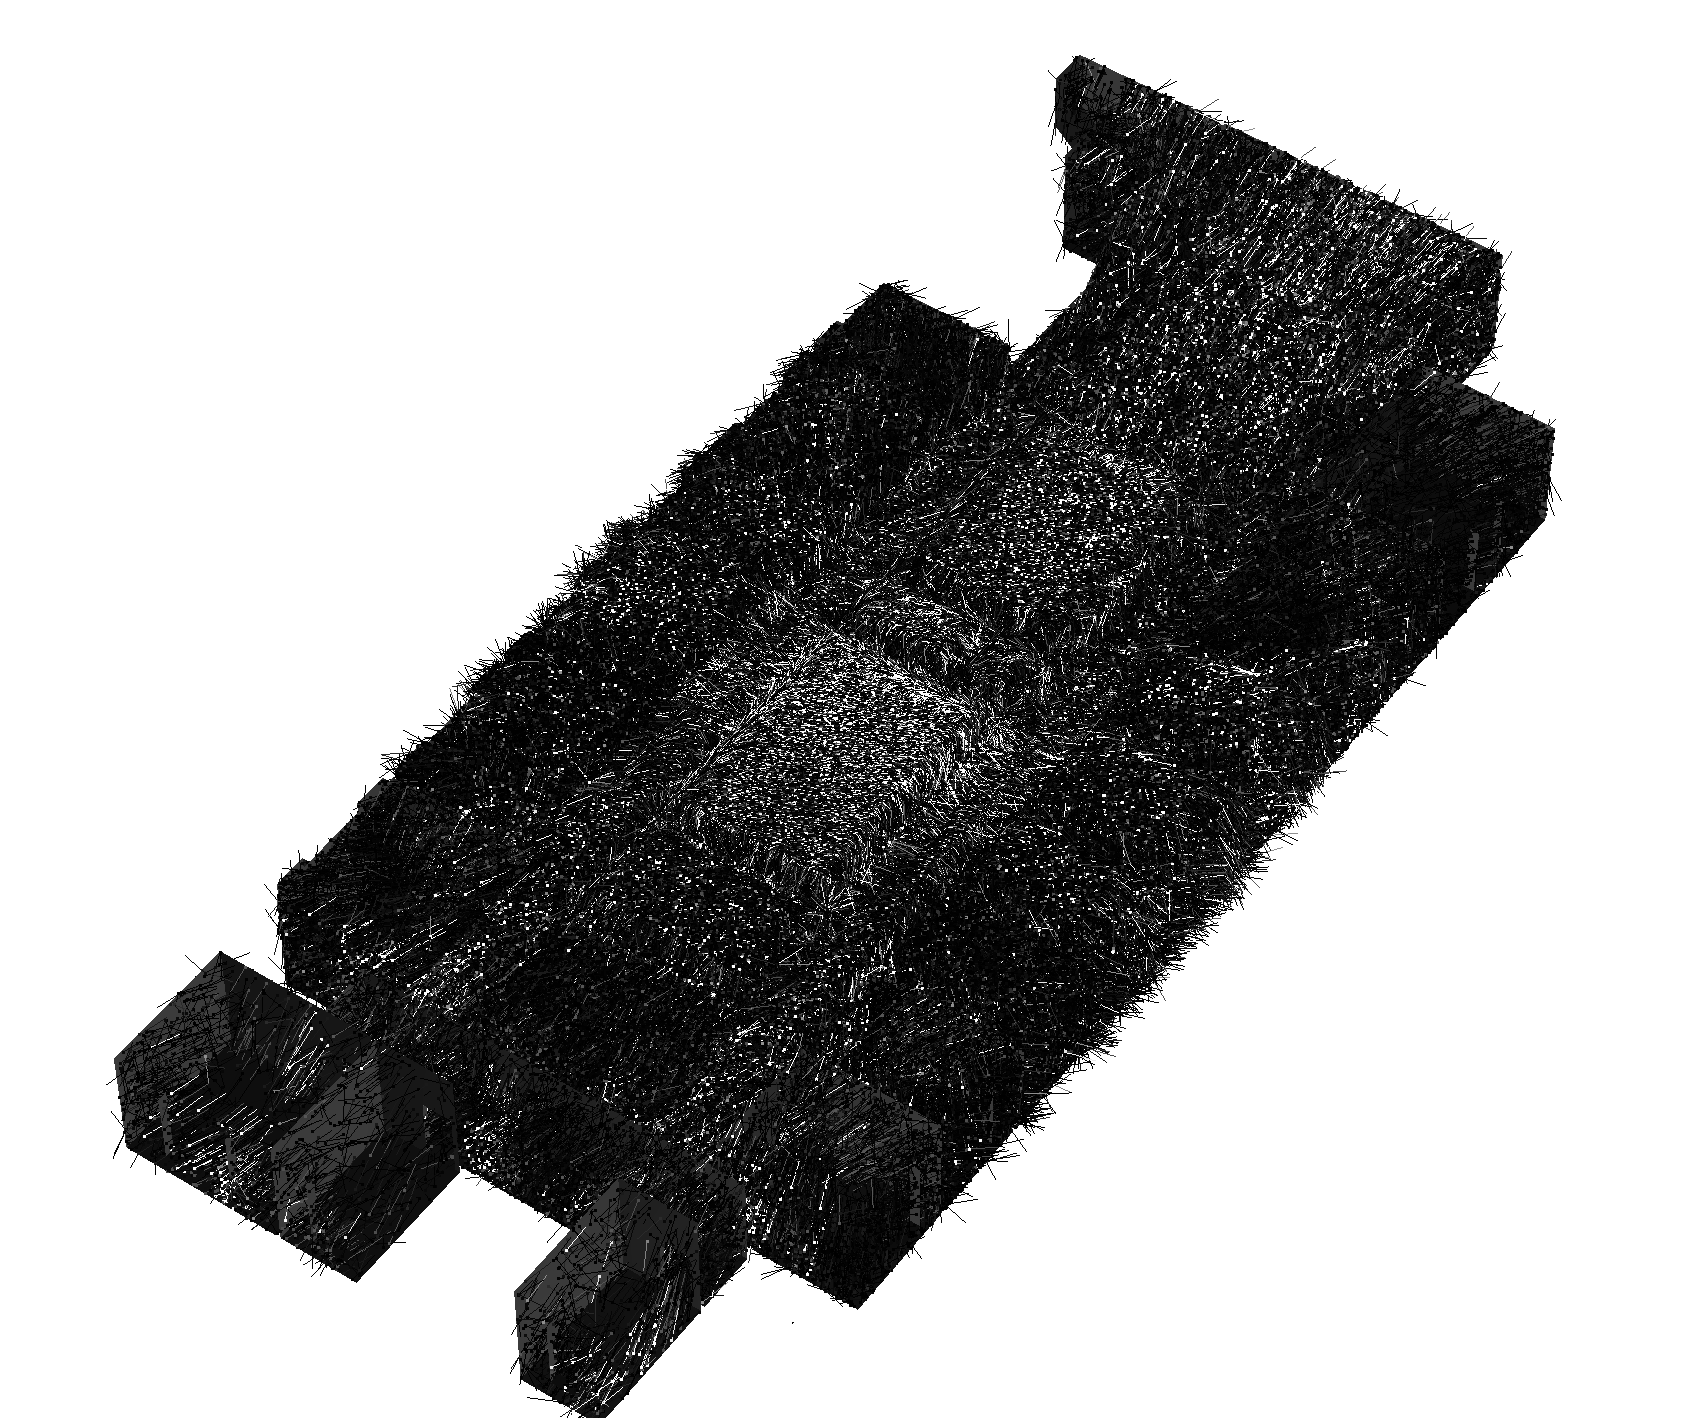
\includegraphics[width=120mm]{trans_photons.png}
\caption{Photon scatter patterns on the first floor of Amos Eaton with
transmissive walls.}
\label{trans_photons}
\end{center}
\end{figure*}

\begin{figure*}
\begin{center}
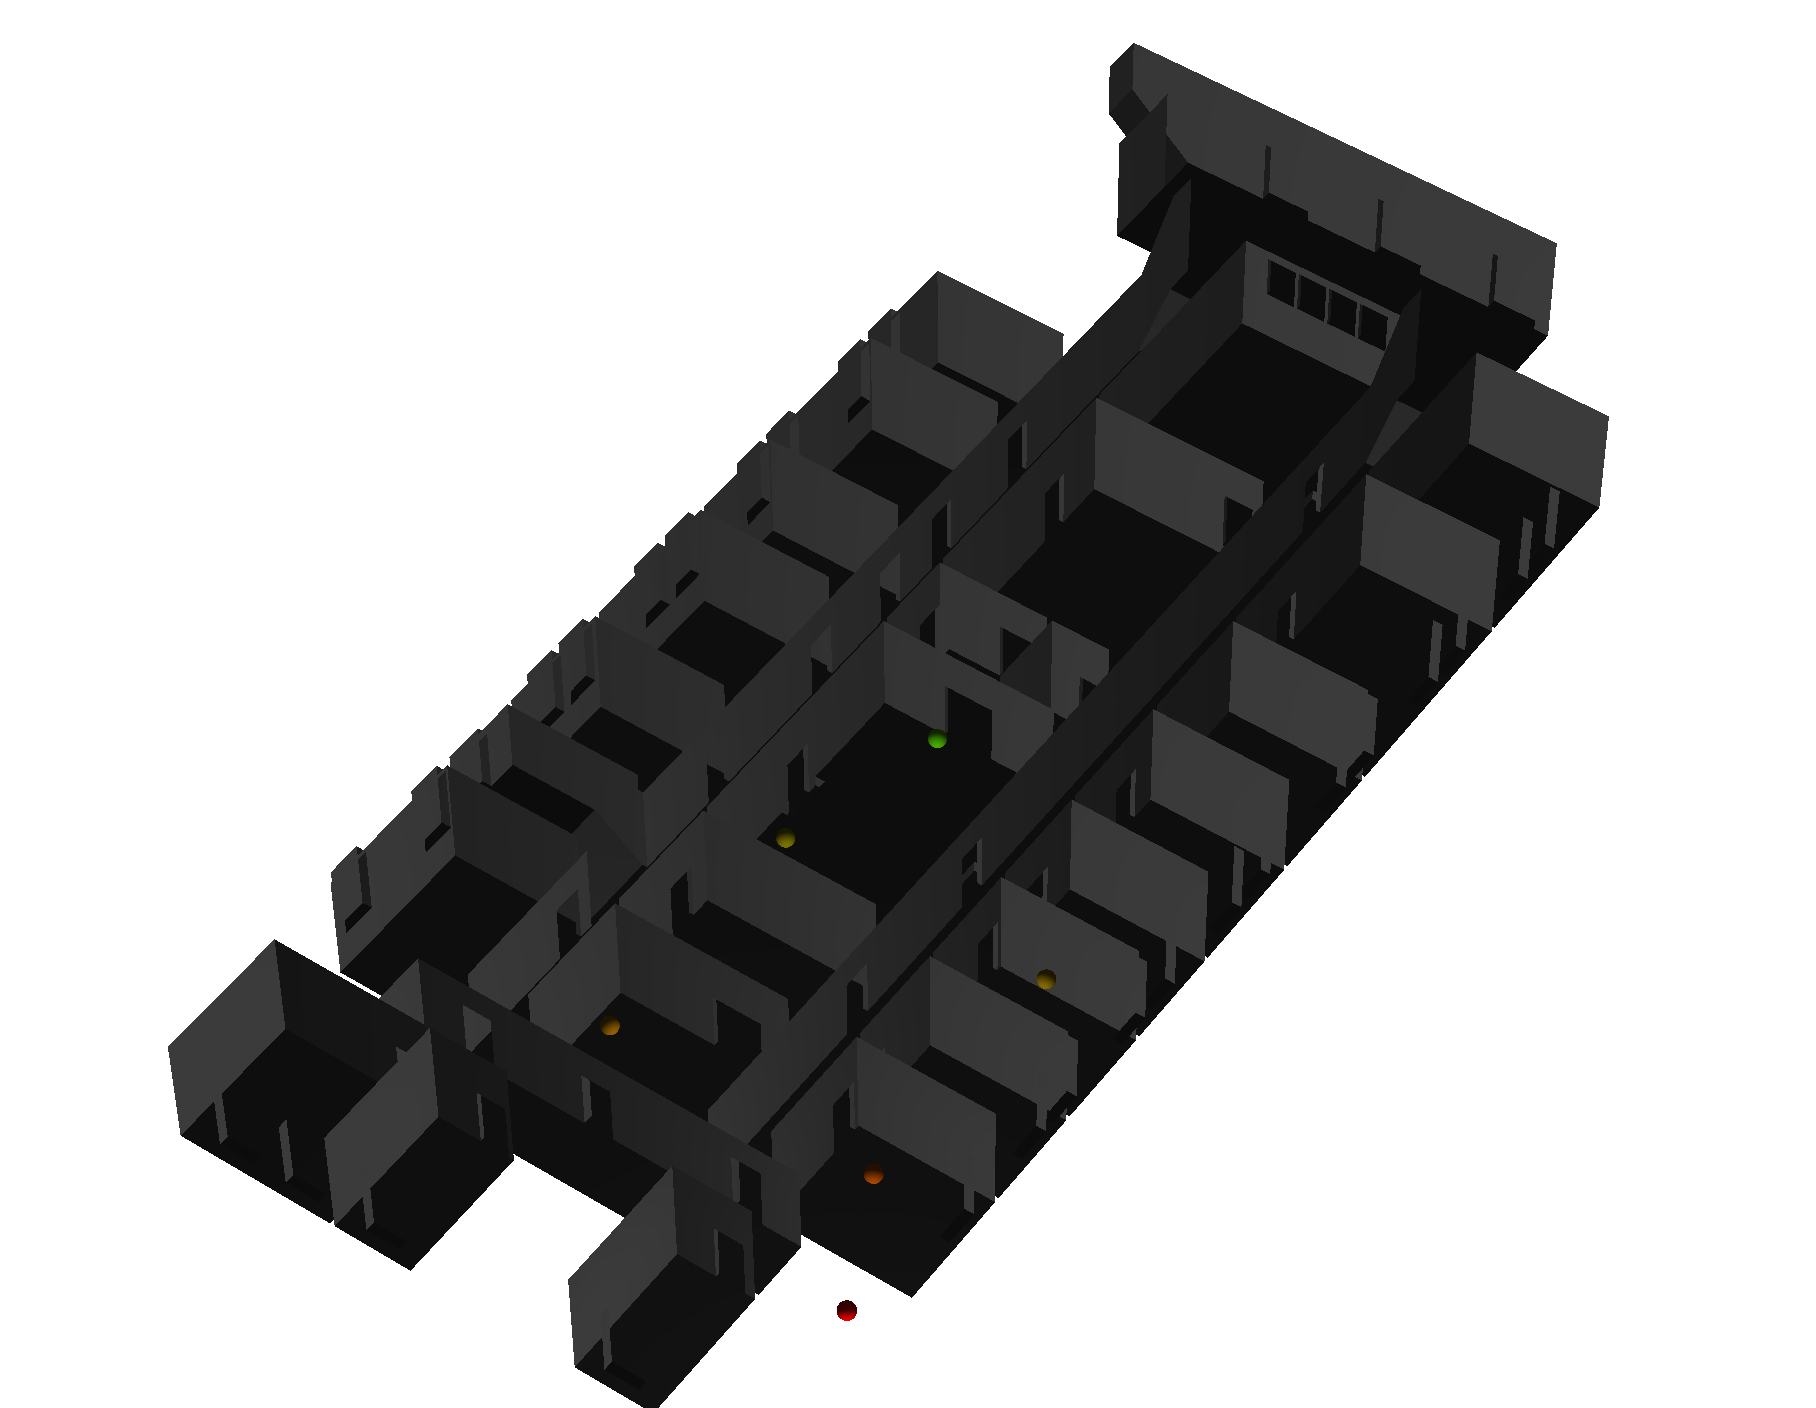
\includegraphics[width=120mm]{trans_sphere.png}
\caption{Bounding spheres at various locations on the first floor of Amos Eaton
with transmissive walls.  Color values range from red (no reception) to green
(good reception).}
\label{trans_sphere}
\end{center}
\end{figure*}

\newpage

\begin{figure*}
\begin{center}
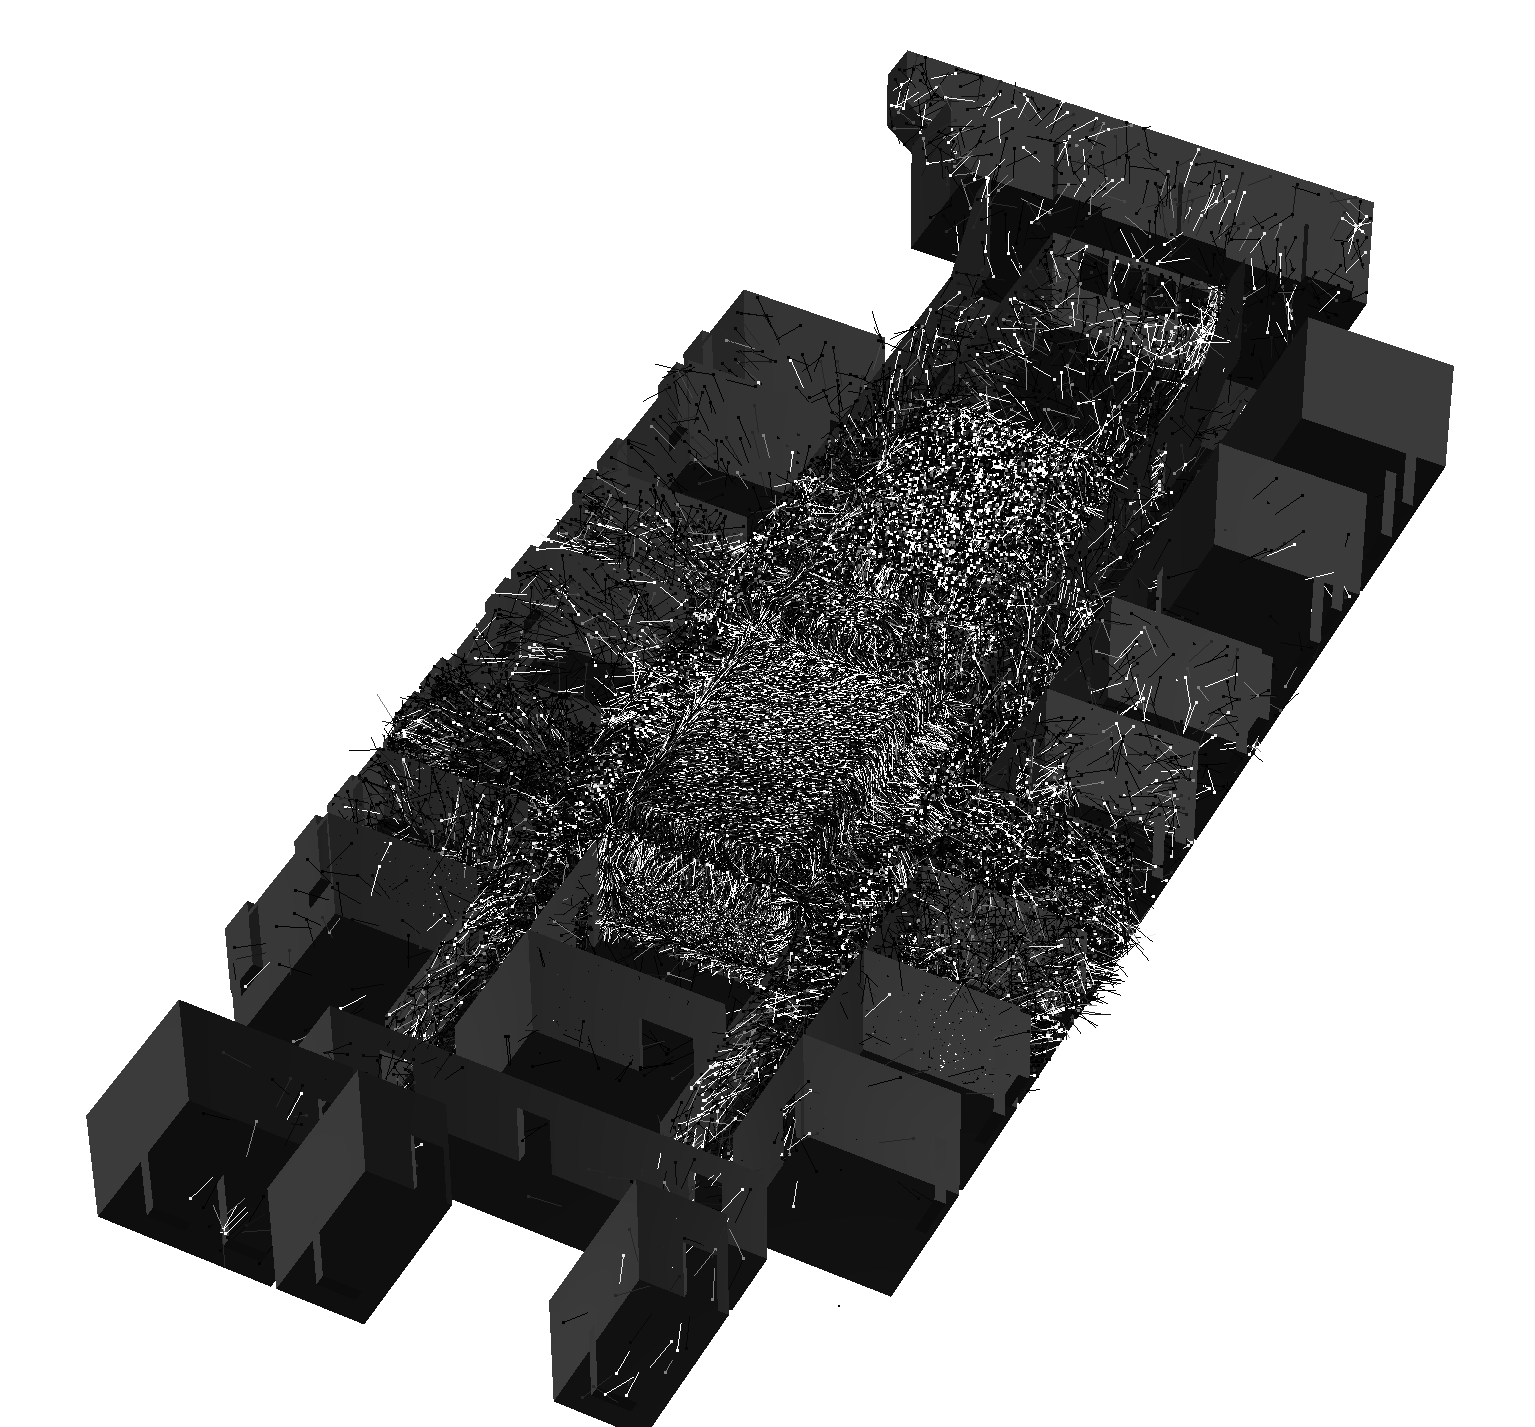
\includegraphics[width=120mm]{no_trans_photons.png}
\caption{Photon scatter patterns on the first floor of Amos Eaton with
non-transmissive walls. The photons do not blanket the entire model as they do
in the transmissive scenario.}
\label{no_trans_photons}
\end{center}
\end{figure*}

\begin{figure*}
\begin{center}
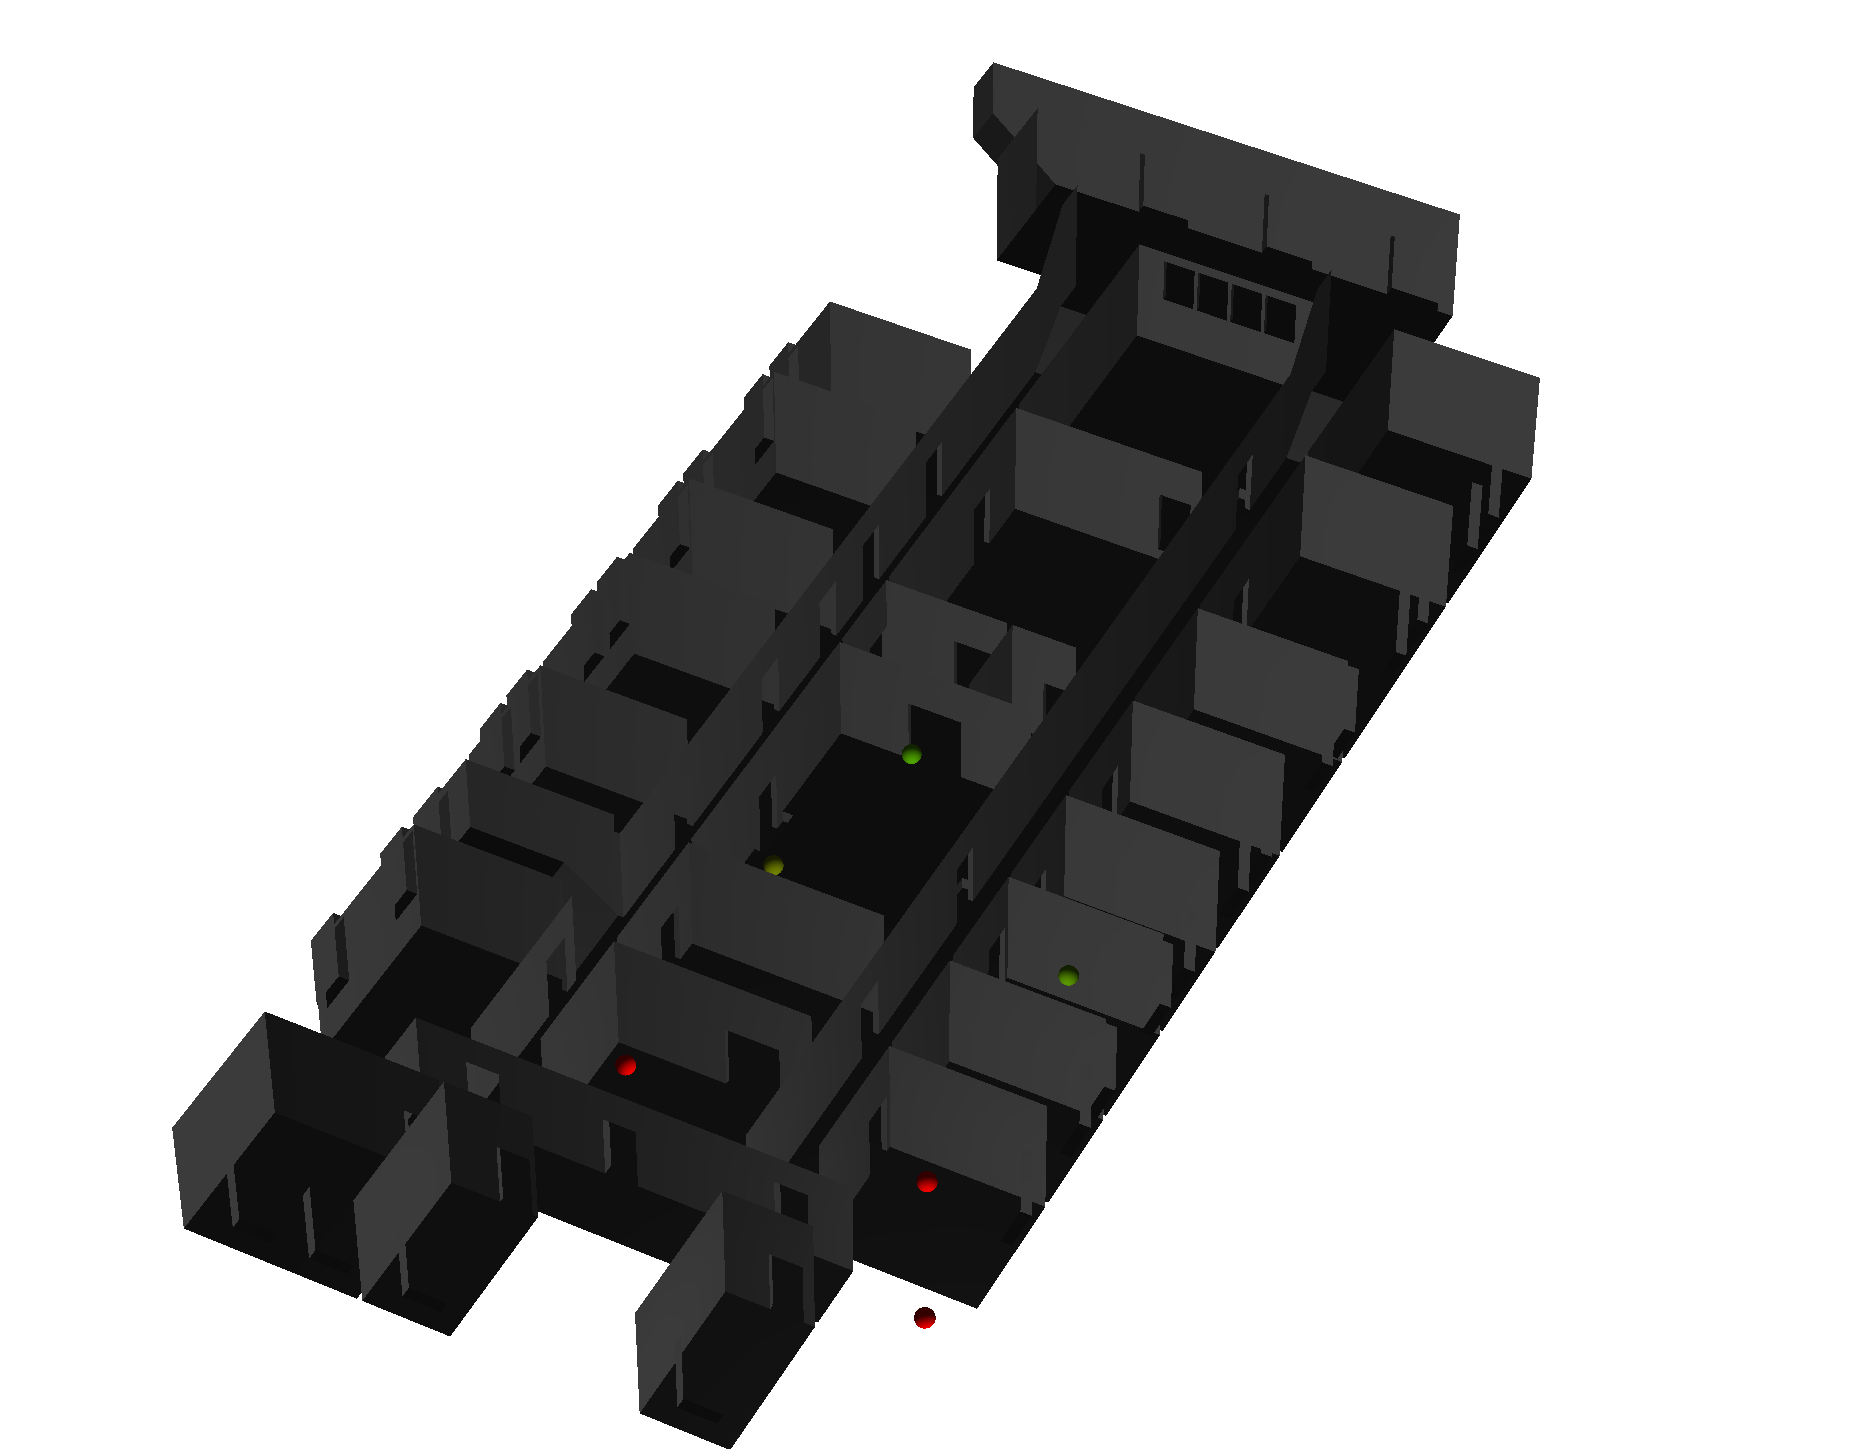
\includegraphics[width=120mm]{no_trans_sphere.png}
\caption{Bounding spheres at various locations on the first floor of Amos Eaton
with non-transmissive walls.  Color values range from red (no reception) to green
(good reception).  Less photons implies weaker signal strength.}
\label{no_trans_sphere}
\end{center}
\end{figure*}

% where ``my-bibliography-file.bib'' is the name of the file with all the 
% BibTeX entries.

% do the biographies...
%\begin{biography}{Gregory L. Plett}
%  A bio with no face...
%\end{biography}

% If you want a picture with your biography, then specify the name of
% the postscript file in square brackets. That is, uncomment the
% following three lines and change the name of "face.ps" to the name of 
% your file.
%\begin{biography}[face.ps]{Gregory L. Plett}
%  A bio with a face...
%\end{biography}

%----------------------------------------------------------------------
% FIGURES
%----------------------------------------------------------------------
% There are many ways to include figures in the text. We will assume
% that the figure is some sort of EPS file.
%
% The outdated packages epsfig and psfig allow you to insert figures
% like: \psfig{filename.eps} These should really be done now using the
% \includegraphics{filename.eps} command.  
%
% i.e.,
%
% \includegraphics{file.eps}
%
% whenever you want to include the EPS file 'file.eps'. There are many
% options for the includegraphics command, and are outlined in the
% on-line documentation for the "graphics bundle". Using the options,
% you can specify the height, total height (height+depth), width, scale,
% angle, origin, bounding box "bb",view port, and can trim from around
% the sides of the figure. You can also force LaTeX to clip the EPS file
% to the bounding box in the file. I find that I often use the scale,
% trim and clip commands.
% 
% \includegraphics[scale=0.6,trim=0 0 0 0,clip=]{file.eps}
% 
% which magnifies the graphics by 0.6 (If I create a graphics for an
% overhead projector transparency, I find that a magnification of 0.6
% makes it look much better in a paper), trims 0 points off
% of the left, bottom, right and top, and clips the graphics. If the
% trim numbers are negative, space is added around the figure. This can
% be useful to help center the graphics, if the EPS file bounding box is
% not quite right.
% 
% To center the graphics,
% 
% \begin{center}
% \includegraphics...
% \end{center}
% 
% I have not yet written good documentation for this, but another 
% package which helps in figure management is the package ieeefig.sty,
% available at: http://www-isl.stanford.edu/people/glp/ieee.shtml
% Specify:
% 
%\usepackage{ieeefig} 
% 
% in the preamble, and whenever you want a figure,
% 
%\figdef{filename}
% 
% where, filename.tex is a LaTeX file which defines what the figure is.
% It may be as simple as
% 
% \inserteps{filename.eps}
%
% or
% \inserteps[includegraphics options]{filename.eps}
% 
% or may be a very complicated LaTeX file. 

\end{document}
